\def\knobshow#1{ \marginpar{ \centering \begin{tikzpicture} \pic
[scale=1.5] {labeleb=#1}; \end{tikzpicture} }}

\def\param#1{{\small \uppercase{#1}}}

\chapter{Paramètres de ventilation}

L'opération du VDR-4 est une tâche complètement différente de
l'opération d'un ventilateur de soins intensifs moderne.

Sur un respirateur moderne, chaque réglage est associé à un seul
paramètre, observable et mesurable. Le microprocesseur de ces appareil
est chargé de contrôler les composantes mécaniques (valve ou turbine)
pour administrer précisément le paramètre programmé par l'utilisateur.

Le réglage des paramètres de ventilation du VDR-4 se fait quant à lui
en ajustant manuellement l'ouverture de valves sur le module de
contrôle.  Les valves du module de contrôle sont identifiées par le
principal paramètre visé par le réglage.  Cependant, à cause du
contrôle entièrement pneumatique de l'appareil, le réglage de
l'ouverture d'une valve entraine presque toujours la modification d'au
moins deux paramètres. Et, conséquemment, chaque paramètre
observable/mesurable (ex. pression, fréquence, ...) est influencé par
plusieurs réglages.

\begin{table}[h] \centering \caption{Code de couleur des réglages}
	\begin{tabular}{ll} \hline Couleur & Catégorie \\ \hline Vert &
		Amplitude de percussion\\ Noir & Basse fréquence\\ Gris & Haute
		fréquence\\ \hline \end{tabular} \end{table}

\section{Amplitude de percussion et pression d'équilibre}

On entend par	\emph{amplitude de percussion} la variation de pression
	résultant de chaque percussion. La pression d'équilibre est quant à
	elle la pression autour de laquelle se stabilisera la pression
	alvéolaire au cour d'une phase du cycle de convection (basse
	fréquence). Les pression moyenne expiratoire et inspiratoire sont
	utilisées comme approximation de ces pressions.

Une amplitude de percussion différente peut être réglée pour chacune
	des trois phases du cycle de convection (basse fréquence). Les
	trois réglages ciblant ces amplitudes sont identifiés par la couleur
	verte sur le module de contrôle. Ceux-ci agissent en modifiant le
	débit injecté à l'arrière du phasitron à chaque percussion, pendand
	chacune de ces trois phases. La modification de ces trois débits
	aura aussi pour effet de modifier, dans la même direction, la
	pression d'équilibre concerné.

L'amplitude de percussion et les pressions d'équilibre seront aussi
	influencés par le rapport \ie des percussions. En laissant peu de
	temps à la pression pour diminuer en chaque percussion, un rapport
	\ie élevé (Ti > Te) favorisera une augmentation des pressions
	d'équilibre mais une diminution de l'amplitude de percussion.

Finalement, la durée du Ti de chaque percussion influencera
	l'amplitude (Ti élevé = amplitude élevée) sans modifier les
	pressions d'équilibre.

\begin{figure}
	\centering
	\tikzsetnextfilename{fig-graphinterraction}
\tikzset{
	vdrwave/.pic={
			\path [pic actions, transform shape] plot [smooth, tension=1] coordinates {
			(0,0) (1,0.7) (2,0) (3,0.9) (4,0) (5,1) (6,0) (7,1) (8,0) (9,1) (10,0)
			(11,2.5) (12,0) (13,2.85) (14,0) (15,3) (16,0) (17,3) (18,0) (19,3) (20,0) 
			(21,1.5) (22,0) (23,1.2) (24,0) (25,1) (26,0) (27,1) (28,0)
			(29,1) (30,0)
		} ;
	},
	amplpic/.pic={
		\begin{scope}[xscale=0.06, yscale=.4]
			\pic [transform shape, draw=black!50] {vdrwave};
			\draw [ultra thick, <->] (6,0) to[ultra thick] (6,3);
		\end{scope}
	},
	pmoy/.pic={
		\begin{scope}[xscale=0.06, yscale=.4, ]
			\path [clip, transform shape] (-15,0) rectangle (22,3);
			\pic [transform shape, draw=black!50] {vdrwave};
			%\draw [ultra thick, <->] (6,0) to[ultra thick] (6,1);
			\draw (20,1.5) -- (6, 1.5) -- (0,2.2) node[left,
			font=\footnotesize] {$\overline{P_{i}}$};
			\draw (10,.5) -- (-2,.5) node[left, font=\footnotesize] {$\overline{P_{e}}$};
		\end{scope}
	}
}

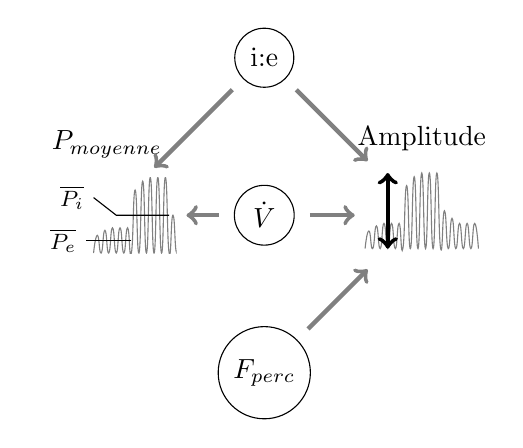
\begin{tikzpicture}	[
		node distance=2cm,
		link/.style={
			->,
			ultra thick,
			black!50,
		},
		indep/.style={
			draw,
			circle,
			outer sep=2mm,
			align=center,
		},
		target/.style={
			scale=0.8,
		},
	]

	\node [matrix,label=Amplitude] (A) {\pic [target] {amplpic};\\};
	\node [left of=A, indep] (D) {$\dot{V}$};
	\node [above of=D, indep] (R) {i:e};
	\node [below of=D, indep] (i) {$F_{perc}$};
	%\node [left of=D] (P) {$P_{moy_{insp.}}$};
	\node [left of=D, matrix,label=$P_{moyenne}$] (P) {\pic
	[target] {pmoy};\\};

	\draw [link] (D) -> (A);
	\draw [link] (R) -> (A);
	\draw [link] (i) -> (A);
	\draw [link] (D) -> (P);
	\draw [link] (R) -> (P);

\end{tikzpicture}

	\caption{Effets du débit, de la fréquence et du ration \ie sur les
	pressions d'équilibre et la'amplitude de percussion.}
\end{figure}

\subsection{Amplitude des percussions à l'inspiration (phase haute)}

Il s'agit du paramètre de base à partir duquel sont réglés les deux
	autres paramètres d'amplitude. Cela signifie qu'une modification de
	ce paramètre entrainera une modification dans la même direction des
	deux autres amplitudes.  Cette amplitude est réglée au moyen de la
	valve identifiée \param{Debit pulse}. Celle-ci contrôle le débit
	injecté à l'arrière du phasitron pendant chaque percussion.
	\knobshow{D	DÉBIT\\PULSÉ}

\subsection{Amplitude des percussions à l'expiration (phase basse)}

L'amplitude des percussions pendant l'expiration convective est réglée
	par comparaison à celle pendant l'inspiration convective. Cela
	signifie qu'une modification de l'amplitude à l'inspiration
	entrainera une modification de l'amplitude à l'expiration. Par
	contre, l'amplitude à l'inspiration ne sera pas affectée par une
	modification de celle à l'expiration. Cette amplitude est réglée au
	moyen de la valve identifiée \param{CPAP oscillante}.
	\knobshow{O CPAP\\OSCILLANTE}

\subsection{Amplitude de percussion augmentée (troisième phase)}

Lorsqu'elle est activée, la troisième phase commence 0,8 seconde après
	le début de l'inspiration convective. Il en résulte une inspiration
	en deux temps. Cette amplitude est réglée au moyen de la valve
	identifiée pression de convection. Ce paramètre n'est pas utilisé
	dans le protocole clinique en vigueur au CHUM.
	\knobshow{C PRESSION DE\\CONVECTION}

\begin{figure}
	\centering
	\begin{tikzpicture}
		\begin{groupplot} [
				group style={
					group size=2 by 1,
					ylabels at=edge left,
				},
				ylabel=$P_{circ.} (hPa)$,
				xlabel=Temps (s),
				width=0.5\textwidth,
				%restrict x to domain=0:5,
				%ymax=40,
				every axis plot post/.style={
					mark=none,
					ultra thin
				}
			]
			\nextgroupplot [title=A]
			\addplot [] table[y index=0, x expr={(\coordindex/512)}] {dat/nocpr.dat};

		 \nextgroupplot [title=B]
			\addplot [] table[y index=0, x expr={(\coordindex/512)}]
			{dat/cpron.dat};
		\end{groupplot}
	\end{tikzpicture}

	\caption[Augmentation de la pression de convection]{La fonction
	\param{Augmentation de la pression de convection} engendre une
	troisième phase débutant 0.8 secondes après le début de
	l'inspiration (Courbe B).}
\end{figure}

\begin{table} \centering \caption{Désignation des contrôles relatifs à
	l'amplitude de percussion.} \begin{tabular}{l l} \hline Paramètre &
		Désignation sur l'appareil\\ \hline Amplitude à l'inspiration
		(phase haute) & \param{DEBIT PULSE}\\ Amplitude à l'expiration
	(phase basse) & \param{CPAP OSCILLANTE}\\ Amplitude augmentée
	(troisième phase) & \param{PRESSION DE CONVECTION}\\ \hline
	\end{tabular} \end{table}

\begin{figure} \centering 
\begin{tikzpicture}[
	fleche/.style={
			line width=0.6mm,
			->,
			shorten >=1mm, 
			shorten <=1mm, 
			font=\small,
			vertvdr!60
		},
		cid/.style={
			above=1.35*\ldist,
			align=center,
			font=\tiny
		},
		ampl/.style={
			fill=vertvdr!72
		},
		marker/.style={
			line width=0.3mm,
			vertvdr!60
		},
		index/.style={
			midway,
			below,
			inner
			sep=0,
			font=\tiny,
			scale=0.8
		},
		aug/.style={
			midway,
			above,
			inner
			sep=1mm,
			font=\tiny,
			scale=0.7
		}
]

\colorlet{vertvdr}{green!50!black}

\newcommand{\pexp}{9.5}
\newcommand{\pins}{35.5}
\newcommand{\arrfirst}{1.69}
\newcommand{\arrseccond}{5.68}
\newcommand{\ldist}{7mm}

	\begin{axis} [
			height=0.80\textheight,
			xtick={0,2,4},
			axis x line=bottom,
			axis y line=left,
			enlarge y limits={0.1, upper},
			enlarge x limits={0.05, upper}
		]

		\addplot [
			restrict x to domain=0:6,
			thin,
			]table[x=time, y=Pao] {dat/simvent1.dat};

		\coordinate (A) at (axis cs:1.445,0.1);
		\coordinate (B) at (axis cs:1.445,\pins);

		\draw [marker] (axis cs:0, \pins) -- (axis cs:6, \pins);
		\draw [marker] (axis cs:4, \pexp) -- (axis cs:6, \pexp);

		\draw [fleche] (axis cs:\arrfirst, 0) -- (axis cs:\arrfirst, \pins)
		coordinate [midway] (A);

		\draw [fleche] (axis cs:\arrseccond, \pins) -- (axis cs:\arrseccond, \pexp)
		coordinate [midway] (B);

		\path (A) ++(axis cs: -.7,0) coordinate (C);
		\path (B) ++(axis cs: -.7,-.4) coordinate (D);

	\end{axis}

	\path (C) pic [ampl] {aknob} 
	node [cid] {DEBIT\\PULSE};

	\draw [<->] (C) ++(\ldist, -\ldist) -- ++(0, 2*\ldist) -- ++(-2*\ldist, 0) 
	node [index] {$\blacktriangledown$}
	node [aug] {AUGMENTER}
	;

	\path (D) pic [ampl] {aknob}
	node [cid] {CPAP\\ OSCILLANTE};

	\draw [->] (D) ++(\ldist, \ldist) -- ++(-2*\ldist, 0)
	node [index] {$\blacktriangledown$}
	node [aug] {AUGMENTER}
	;

\end{tikzpicture}

\caption{Interaction entre les paramètres d'amplitude.}
\label{figinterampl} \end{figure}

\section{Paramètres de cyclage à haute fréquence}

Les valves contrôlant le cyclage à haute fréquence sont identifiées
	par la couleur grise sur le module de contrôle.  Bien que les deux
	boutons permettant de régler le cyclage à haute fréquence soient
	désignés \param{Frequence de percussion} et \param{RATIO} i:e sur
	l'appareil, il s'avère que chacun de ces deux \knobshow{i FRÉQUENCE
	DE\\PERCUSSION} réglages
	influence la fréquence.  En fait, le bouton \param{Frequence de
	percussion} modifie le temps inspiratoire des percussions sans
	modifier le ratio i:e. Il en résulte donc une modification de la
	fréquence avec un ratio i:e constant.  Quant au bouton \param{RATIO}
	i:e, il ajuste le ratio i:e des percussions sans modifier le temps
	inspiratoire. Il en résulte qu’une modification du ratio i:e modifie
	aussi la fréquence de percussion.
	\knobshow{e RAPPORT \ie}

\section{Paramètres de cyclage à basse fréquence}

Le cyclage à basse fréquence se règle en ajustant un temps
	inspiratoire et un temps expiratoire.  La fréquence et le ratio
	inspiration: expiration résulteront des temps inspiratoire et
	expiratoire réglés. Les valves contrôlant le cyclage à basse
	fréquence sont identifiées par la couleur noire sur le module de
	contrôle.

\section{PEP non oscillante}

La fonction PEP non oscillante (DEMAND CPAP / PEEP) est identifiée par
	un bouton de couleur jaune.  Cette fonction est destinée à réduire
	le travail respiratoire lors d'essai de respiration spontanée. Elle
	est généralement désactivée lors de la percussion. Lorsqu'elle est
	activée, un débit continu est injecté dans le phasitron. Ce débit,
	qui sera amplifié par le phasitron, facilite l’inspiration et
	maintient une pression positive à l'expiration (en maintenant le
	tube de venturi en position partiellement avancée).  

\section{Autres paramètres}

\subsection{Pression de travail}

La pression de travail est la pression à laquelle les gaz entrent dans
	le circuit de logique pneumatique. Celle-ci influence à la fois
	l'amplitude des percussions et les paramètres de cyclage. Chez
	l'adulte, on utilise généralement la pression la plus élevée pouvant
	être atteinte (plus ou moins 40 \psi, selon la source d'alimentation
	en gaz pressurisé).


\subsection{Nébulisation}

Active ou désactive le débit destiné à actionner le nébuliseur (plus
ou moins 20 l/min). Actif même lorsque la percussion est arrêtée. 

\subsection{Marche arrêt}

S'applique à la percussion seulement. Toutes les autres fonctions
(nébulisation, PEP non percussive, monitorage) demeurent actives.
\marginpar{%
	\centering
	\begin{tikzpicture}
		\pic {master};
		\node [above=1cm, font=\scriptsize] {INTERRUPTEUR};
	\end{tikzpicture}}

\section{Interactions des paramètres}

Pour faire une règle simple, on peut dire, sans trop exagérer, que
n'importe quel paramètre peut potentiellement influencer n'importe
quel autre paramètre. 

\subsection{Paramètres influençant le cyclage}

Étant donné que l'alternance entre les inspirations et les expirations
des percussions (cyclage haute fréquence)  est contrôlé par des
cartouches pneumatiques, tout paramètre influençant la pression
disponible pour actionner les cartouches peut influencer la fréquence
des percussions et leur ratio i:e.  Parmi ces paramètres, on compte
entre autres:

\begin{itemize} \item La pression de travail, \item La \fio, \item Le
réglage d'amplitude des percussions (\param{debit pulse}).
\end{itemize}

Le même principe s'applique au cyclage à basse fréquence (temps
inspiratoire et expiratoire convectif).

\subsection{Influence du ratio i:e des percussions sur les pressions
de ventilation}

Le ratio inspiration: expiration (i:e) des percussions a une grande
influence sur les pressions de ventilation. Plus le ratio i:e est
élevé, plus les pressions serons élevées.

\section{Séquence des réglages}

\begin{figure*} \centering
\begin{tikzpicture}

	\pic [name=VDR, black!60, scale=0.8] {vdr};

	\begin{scope}[
		every node/.style={
			color=black,
			}
			]
	\node (1) at (VDR-e) {1};
	\node (2) at (VDR-i) {2};
	\node (3) at (VDR-F) {3};
	\node (4) at (VDR-O) {4};
	\node (5) at (VDR-I) {5};
	\node (6) at (VDR-E) {6};
	\end{scope}

	\begin{scope}[
		every node/.style={
			yshift=8mm,
			align=center,
			scale=0.5
			}
			]
	\node at (VDR-e) {RAPPORT\\i/e};
	\node at (VDR-i) {FREQUENCE\\DE PERCUSSION};
	\node at (VDR-F) {DEPIT\\PULSE};
	\node at (VDR-O) {CPAP\\OSCILLANTE};
	\node at (VDR-I) {TEMPS\\INSPIRATOIRE};
	\node at (VDR-E) {TEMPS\\EXPIRATOIRE};
	\end{scope}

	\begin{scope}[
		every path/.style={
			black,
			opacity=0.80,
			line width=0.7mm,
			->
			},
			]
	\draw [] (1) to (2);
	\draw [bend left=27] (2) to (3);
	\draw [bend left=60] (3) to (4);
	\draw [bend left=45] (4) to (5);
	\draw [bend left=45] (5) to (6);
	\end{scope}

\end{tikzpicture}
 \caption{Séquence de réglage
des paramètres.} \end{figure*}

En raison des interactions entre les différents réglages, il est
judicieux de régler en premier les paramètres ayant beaucoup
d'influence sur les autres réglages, ou influençant plusieurs autres
réglages.

Ainsi, avant d'effectuer quelque réglage que ce soit, on s'assurera
que la pression de travail est réglée à 40 lb/po\textsuperscript{2} et
que la nébulisation est en fonction. On s'assurera aussi que la PEP
non oscillante et l'augmentation des pressions de convection
(3\textsuperscript{e} phase) sont désactivées (tourné complètement en
sens horaire).

Ensuite, étant donné que le rapport \ie\ des percussions (haute
fréquence) influence à la fois la fréquence de percussion et
l'amplitude des percussions (donc les pressions de ventilation), il
est judicieux d'ajuster ce paramètre en tout premier lieu.

Une fois le rapport \ie\ des percussions ajusté,~le temps inspiratoire
des percussions peut être ajusté à n'importe quel moment pour régler
la fréquence de percussion.

Pour les paramètres d'amplitude de percussion, l'amplitude des
percussions pendant l'inspiration influence celle pendant
l'expiration.  Il convient donc de toujours ajuster la pression
inspiratoire avant la pression expiratoire.

Finalement, les pressions de ventilation ayant une influence sur le
temps inspiratoire et expiratoire de la convection (basse fréquence),
on attendra d'avoir ajusté les pressions de ventilation avant de
régler avec précision ces deux paramètres.
